\documentclass[a4paper, 11pt]{article}
\usepackage{geometry}
\geometry{letterpaper, margin=1in}
\usepackage{amsmath}
\usepackage{amssymb}  
\usepackage{amsthm}
\usepackage{ulem} 
\usepackage{graphicx}
\usepackage{enumitem} 
\graphicspath{ {images/} }


\newtheorem*{theorem}{Theorem}

\begin{document}
%Header-Make sure you update this information!!!!
\noindent
\large\textbf{Thermal Physics - PH441} \hfill \textbf{John Waczak} \\
\normalsize Day 13 \hfill  Date: \today \\

	
		
\subsection*{Some midterm review} 
	It will be in class, normal 50 minute, closed notes exam. Online there is a short list of equations we should have memorized. 
		\begin{align*}
			dU &= TdS - pdV \\ 
			F &= U - TS \\ 
			dF &= -SdT - pdV \\ 
			P_i &= \frac{e^{-\beta E_i}}{Z} \\ 
			Z &= \sum\limits_\mu e^{-\beta E_\mu} \\ 
			U &= \langle E \rangle = \sum\limits_\mu E_\mu P_\mu \\ 
			F &= -kT\ln Z
		\end{align*}
		
		
\subsection*{Chemical Potential}
	For some motivation consider the system of a round, solid Earth with a gaseous atmosphere. Now imagine we want to explore the properties of the atmosphere as a function of the distance from the surface of the Earth (h). \\
	
	\noindent So far we have tried to drill that a microstate is the energy eigenvalue solution to a quantum mechanical problem. So solving this kind of problem is yelling \textit{CLASSICAL APPROXIMATION} at you. Quantum mechanically we cant treat momentum and position differently. In classical approximations you can so we take $(q_i, p_i)$. So think of a microstate as a volume in phase space. Imagine the case of a simple harmonic oscillator. In phase space this would 
	trace out a circle. \textbf{Liouville's theorem} dictates that volumes in phase space never change. Think of this kind of like an uncertainty principle. 
		\begin{figure}[!hbt]
			\centering
			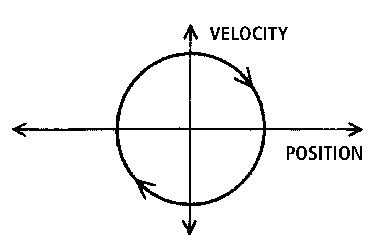
\includegraphics[width=0.4\columnwidth]{sho_phaseSpace}
		\end{figure}
		
	\noindent Having considered all of that what is $P(\vec{p},\vec{r})$? 
		\begin{align*}
			P(\vec{p}, \vec{r})&= \frac{e^{-\beta (\frac{p^2}{2m}+mgh)}}{Z}\\
			Z &= \int d^3p \int d^3 r e^{-\beta (\frac{p^2}{2m}+mgh)}
		\end{align*}
	
	\noindent Here we have considered the ph211 uniform gravitational field with potential $U = mgh$. We could try and solve this to some degree of success, but we should be able to separately treat the top and bottom of the atmosphere (because they are observed to be very different) which leads us to discussing the chemical potential. \\ 
	
	\noindent Imagine a box at high atmosphere and a box at low atmosphere. We imagine particles to move freely from one box to the other a.k.a. \textbf{Diffusive equilibrium}. How do we deal with allowing particles to go from one state to another? First let's start by just imagining two boxes with some sort of pipe connecting them that allows transport. Thermodynamics tells us that at equilibrium, $T_A = T_B$. There should be something else though that equilibrates if we allow the particles to move between the systems. We will call this quantity the chemical potential giving us that at equilibrium:	
		\begin{equation*}
			\mu_A = \mu_B 
		\end{equation*}
		
	\noindent If it helps, you could also imaging a single volume with some kind of permeable membrane that is free to move which would lead to $P_A = P_B$ (a rough translation of Newton's second law). \\
	
	\noindent Let's talk through (hand-waivey) what the chemical potential must be. Recall from our discussion of $F$, we said that if you keep something at fixed temperature, $F$ is the thing that's minimized. So to try and minimize the Helmholtz free energy for our new system that allows transport we would have:	
		\begin{align*}
			\Big(\frac{\partial F_{tot}}{\partial N_A}\Big)_{T,N} &= 0\\
			\Big(\frac{\partial F_A}{\partial N_A}\Big)_T + \Big(\frac{\partial F_B}{\partial N_B}\Big)_T\Big(\frac{\partial N_B}{\partial N_A}\Big)_N &= 0 \\
			\Rightarrow \mu_A &= \Big(\frac{\partial F_A}{\partial N_A}\Big) = \Big(\frac{\partial F_B}{\partial N_B}\Big) = \mu_B 
		\end{align*}
	
	So if you believe that the Helmholtz free energy is the \textit{thing} that is minimized at thermal equilibrium, then we can redefine our Helmholtz as a function that allows N to change yielding: 
		\begin{align*}
			F &= F(T,V,N) \\ 
			dF &= -SdT -pdV + \mu dN \\ 
			dU &= TdS - pdV + \mu dN
		\end{align*}
	Which leads to the alternative definition
		\begin{align*}
			\mu &= \Big(\frac{\partial U}{\partial N}\Big)_{V,S}
		\end{align*}
	
	\noindent We just argued that two things that are in diffusive equilibrium must have equal chemical potentials. The chemical potential, looking at out internal energy, tells us how much energy is required to add a new molecule. There are two types to consider though. An \textbf{External Chemical Potential} is stuff that contributes to the chemical potential (like the work required to lift a molecule to a height h) that do not depend intrinsically on the type of substance i.e. not an inherent property of the substance. The \textbf{Internal Chemical Potential} will depend on the problem at hand. When we write $\mu$, we mean the total chemical potential. This can lead to problematic minus signs but don't be afraid! We'll just trudge along and see how this works. 
		
		
\subsection*{Example: An ideal gas} 
	Recall from last week that for an Ideal gas, the Helmholtz was given as:
		\begin{align*}
			F &= NkT\ln(\frac{N}{Vn_Q})-NkT \\ 
			\text{where } n_Q &= \Big(\frac{mKT}{2\pi \hbar^2}\Big)^{3/2}
		\end{align*}
	\noindent Find the chemical potential.
		\begin{align*}
			\mu &= \Big(\frac{\partial F}{\partial N}\Big) \\ 
				&= kT\ln\Big(\frac{N}{Vn_Q}\Big)-kT+kT \\ 
				&= kT\ln\Big(\frac{N}{Vn_Q}\Big) \\
				&= kT\ln\Big(\frac{n}{n_Q}\Big) \quad \text{where } n \text{ is number denisty} 
		\end{align*}
		
	\noindent Using Roundy's trick, we could have done this easier by observing that $\ln\Big(\frac{N}{Vn_Q}\Big) = \ln(N)-\ln(V)-\ln(n_Q)$. The second terms are constants for the $\partial_N$ derivative and so go to zero making your life easy. With some slight trickery we can conclude something interesting: 
		\begin{align*}
			n &= n_Q e^{\beta \mu_{int}}
		\end{align*} 
	
	\noindent For our atmosphere we have the following: 
		\begin{align*}
			\mu_{ext} &= mgh \\ 
			\mu_{tot} &= \mu_{int} + mgh \\ 
			\Rightarrow n(h) &= n_Qe^{\beta (\mu_{tot}-mgh)}
		\end{align*}
	\noindent Which gives us the familiar result that density decreases with the height. $\mu_{tot}$ is just a number... fret not. 
\end{document}




























